\documentclass{article}
\usepackage[utf8]{inputenc}
\usepackage{enumitem}
\usepackage{tikz}

% Mots-clés des algorithmes en français
\usepackage[french,onelanguage]{algorithm2e}

% Nom et caption de l'algorithme au dessus
\makeatletter
\renewcommand{\@algocf@capt@plain}{above}% formerly {bottom}
\makeatother

% Début
\title{Complexité et Calculabilité 2019/20\newline Devoir maison}
\author{Robin Navarro, Adrien Boitelle}
\date{Octobre 2019}

\begin{document}

\maketitle

\section{Définition du problème Distance commune}

\begin{enumerate}
\item 
Le certificat pour notre vérificateur est un entier n. Le certificat est de taille polynomiale.\newline
Notre vérificateur va dans un premier temps vérifier si n n'est pas plus grand que le nombre de sommet dans chaque graphe. S'il l'est, on peut répondre non. Si nous avons N graphes, pour chaque graphe la lecture du nombre de sommet en $\mathcal{O}(|V|)$. La complexité de cette étape est donc $\mathcal{O}(N * max|V|)$, ce qui est polynomial. \newline

Ensuite, on regarde pour chaque graphe s'il existe un chemin de taille n  allant de s à t. Pour ce faire, nous effectuons un parcours en profondeur sur chaque graphe en partant de s, qui ne parcoure qu'une profondeur maximale de taille n, et qui s'arrête si à cette profondeur il rencontre le sommet t. Si en parcourant tout le graphe avec des chemins de taille maximum n nous ne rencontrons pas t, nous pouvons répondre non. Si après avoir réalisé cette opération nous avons bien atteint t dans tous les graphes, nous pouvons répondre oui.\newline

Dans cette dernière étape, pour un graphe i, le parcours en profondeur est en $\mathcal{O}(|V_i| + |E_i|)$. Comme nous avons N graphes, la complexité devient $\mathcal{O}(N * (max|V_i| + max|E_i|))$, ce qui est polynomial. Nous avons un vérificateur polynomial, avec des certificats polynomiaux, Distance commune est donc un problème appartenant à la classe NP.
\end{enumerate}
\newpage
\section{Cas particulier acyclique}

\begin{enumerate}
\item 

Pour notre algorithme, nous allons utiliser pour chaque graphe un tableau de taille $n - 1$, n étant le nombre de sommets du graphe, et commençant à l'index 0. Chaque case du tableau contientra une liste. A la fin, pour l'index $i, 0 \le i \le n - 1$, le tableau contiendra tous les sommets accessibles à une distance i de s. Pour tous les index i contenant t dans leur liste, on sait qu'il existe un chemin de taille i de s à t.
Nous allons utiliser une fonction pour réaliser ce calcul pour un graphe donné.

\begin{algorithm}[H]
\KwData{V, E, s, t}
\KwResult{Toutes les longueurs de chemins possibles entre s et t}
\BlankLine

nombreSommets = $|V|$\;
t = tableau de taille nombreSommets - 1\;
\BlankLine

\For{i = 1 à n - 1}{
    t[i] = list\_vide()\;
}
t[0] = \{s\}\;
\BlankLine

\For{i = 0 à nombreSommets - 2} {
    \For{Tout sommet u dans t[i]}{
        \For{Tout voisin v de u}{
            \If{v n'est pas dans t[i + 1]}{
                ajouter v à t[i + 1]\;
            }
        }
    }
}
\BlankLine

resultat = liste\_vide()\;
\For{i = 0 à nombreSommet - 1}{
    \For{Tout sommet u dans t[i]}{
        \If{u == s}{
            ajouter i à resultat\;
            break\;
        }
    }
}
\BlankLine

retourner resultat\;
\caption{Fonction Distances\_s\_t(V, E, s, t)}
\end{algorithm}



\newpage
Nous utilisons cette fonction pour chaque graphe, et nous essayons de trouver une valeur de n commune pour tout les graphes.

\begin{algorithm}
\KwData{G1= (V1, E1, s1, t1), ... , GN= (VN, EN, sN, tN)}
\KwResult{Retourne s’il existe un entier n tel que chacun des graphes G1,... , GN possède un chemin simple et valide de longueur n}

N = nombre de paramètres\;
t = tableau de taille N\;

\For{i allant de 0 à N - 1}{
    t[i] = Distances\_s\_t($V_i$, $E_i$, $s_i$, $t_i$)\;
}
\BlankLine

\For{Tout d dans t[0]}{
    continuer = Vrai\;
    \For{i allant de 1 à N - 1}{
        \If{d n'est pas dans t[i]}{
            continuer = Faux\;
            break\;
        }
    }
    \BlankLine
    
    \If{continuer == Vrai}{
        retourner Oui\;
    }
}
\BlankLine

retourner Non\;
\caption{Distance Commune (G1= (V1, E1, s1, t1), ... , GN= (VN, EN, sN, tN))}
\end{algorithm}
Nous allons tout d'abord calculer la complexité de la fonction Distances\_s\_t. Dans la suite, n est défini comme étant le nombre de sommets du graphe passé en paramètre de la fonction ayant le plus grand nombre de sommets.
\begin{itemize}
    \item 
    Calculer $|V|$ et initialiser le tableau se font en $\mathcal{O}(n)$.
    \item
    Imbrication de boucle for:
    \begin{itemize}
        \item 
        Première boucle allant de 0 à n - 2: $\mathcal{O}(n)$.
        \item
        Deuxième boucle $\forall$ sommet u dans t[i]:\newline
        Dans le pire cas, chaque sommet est relié à tous les autres. Mais comme chaque sommet ne peut être présent qu'une seule fois dans une list, c'est en $\mathcal{O}(n)$
        \item
        Troisème boucle $\forall$ voisin de u. Comme expliqué dans la deuxième boucle, il y a au maximum n - 1 voisins. Donc nous sommes en $\mathcal{O}(n)$.\newline Mais dans cette boucle, nous allons parcourir la liste pour voir si le sommet n'y est pas déjà. Au pire cette liste contient n - 2 sommets, donc $\mathcal{O}(n)$.
    \end{itemize}
    Nous avons donc une complexité de $\mathcal{O}(n^4)$ pour cette partie. 
    \item
    Il reste ensuite la recherche du résultat : 
    \begin{itemize}
        \item 
        Première boucle pour i allant de 0 à n - 1 : $\mathcal{O}(n)$.
        \item
        Deuxième boucle $\forall$ u dans t[i] : $\mathcal{O}(n)$. Le corps de cette boucle est en $\mathcal{O}(1)$.
    \end{itemize}
    Nous avons donc une complexité de $\mathcal{O}(n^2)$ pour cette partie.
\end{itemize}
La complexité de Distances\_s\_t est donc $\mathcal{O}(n^4)$.

Il reste la complexité de Distance commune. Ici N est le nombre de graphes passés en paramètre.
\begin{itemize}
    \item 
    Pour chaque graphe on appel Distance\_s\_t: $\mathcal{O}(N * n^4)$.
    \item
    \begin{itemize}
        \item 
        $\forall$ d dans t[0]: Comme nous avons au plus un chemin de taille n - 1, $\mathcal{O}(n)$
        \item
        pour i allant de 1 à N - 1: $\mathcal{O}(N)$. Dans cette boucle, on vérifie si d est présent dans t[i].
        Cette opération parcourt au pire tous les éléments, donc $\mathcal{O}(n)$.
    \end{itemize}
    Nous avons donc une complexité en $\mathcal{O}(N * n^2)$ pour ces boucles imbriquées.
\end{itemize}
La complexité totale de cet algorithme est donc : $\mathcal{O}(N * n^4)$. C'est donc un algorithme polynomial en la taille de l'entrée.
\item
Cet algorithme ne peut être utilisé dans le cas avec cycle, car l'algorithme cherche toutes les valeurs de n possibles. Or avec un cycle, on peut avoir un nombre de n infini en passant plusieurs fois dans le cycle. L'algorithme ne s'arrêterait jamais.

\item 
Si on change le problème en autorisant les chemins non simples, on peut alors construire des graphes tels que la distance n minimum soit exponentielle en la taille du nombre de graphe en paramètre. Pour tout graphe $G_i, 1 \le i \le N$, on crée le sommet s relié à une suite de $2^i$ sommets intermédiaires reliés entre eux. Le dernier de ces sommets est relié à t. On rajoute une boucle sur s. Ainsi, la longueur minimale pour parcourir tous les sommets intermédiaires dans le graphe $G_N$ est $2^N - 1$. Il faut rajouter l'arête pour aller de s au premier de ces sommets intermédiaires, et une autre pour aller du dernier vers t. On obtient en tout un chemin minimum de taille $2^N + 1$. La boucle sur s nous permet de pouvoir atteindre un chemin de cette taille dans tous les graphes plus petits en "pompant" sur cette boucle.

\newpage
Pour $G_1$, nous construisons ce graphe :
\begin{tikzpicture}

\node (n1) at (1, 10) {s};
\node (n2) at (3, 10) {$s_1$};
\node (n3) at (5, 10) {t};

\draw (n1) edge[->] (n2);
\draw (n2) edge[->] (n3);
\draw (n1) edge[loop above] (n1);


\end{tikzpicture}
\newline

Pour tout graphe $G_i$, nous avons donc :
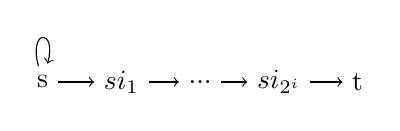
\begin{tikzpicture}

\node (n1) at (1, 10) {s};
\node (n2) at (2, 10) {$si_1$};
\node (n3) at (3, 10) {...};
\node (n4) at (4, 10) {$si_{2^i}$};
\node (n5) at (5, 10) {t};

\draw (n1) edge[loop above] (n1);
\draw (n1) edge[->] (n2);
\draw (n2) edge[->] (n3);
\draw (n3) edge[->] (n4);
\draw (n4) edge[->] (n5);


\end{tikzpicture}
\newline
Pour le dernier graphe $G_N$, nous construisons donc ce graphe :
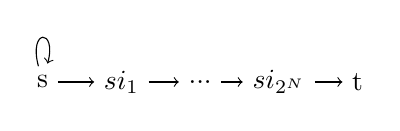
\begin{tikzpicture}

\node (n1) at (1, 10) {s};
\node (n2) at (2, 10) {$si_1$};
\node (n3) at (3, 10) {...};
\node (n4) at (4, 10) {$si_{2^N}$};
\node (n5) at (5, 10) {t};

\draw (n1) edge[loop above] (n1);
\draw (n1) edge[->] (n2);
\draw (n2) edge[->] (n3);
\draw (n3) edge[->] (n4);
\draw (n4) edge[->] (n5);

\end{tikzpicture}, possèdant $N$ sommets intermédiaires.\newline
Le chemin le plus court possible est bien $s \rightarrow si_1 \rightarrow ... \rightarrow si_{2^N} \rightarrow t$, de taille $\mathcal{O}(2^N)$.
\end{enumerate}

\section{Réduction de Distance commune vers SAT}

\begin{enumerate}
\item \begin{enumerate}[label=(\alph*)]
\item
Comme nous considérons des chemins simples, c'est-à-dire passant une seule fois par chaque sommet, on va prendre comme valeur de k maximale le plus grand chemin que l'on puisse construire dans le graphe le plus petit que nous ayons en entrée. \newline
Soit $G_{min}$ le plus petit graphe donné en entrée, le chemin simple le plus long est lorsque tout les sommets de $G_{min}$ sont les uns à la suite des autres. Soit n le nombre de sommet, alors ce chemin est de taille n - 1.\newline
$k_{max}$ est donc de taille $|V_{min}| - 1$.\newline

\item 

Nous avons découpé notre formule en 5 sous-formules.
\begin{enumerate}
    \item
    Le chemin de chaque graphe $G_i$ commence par $s_i$ et finit par $t_i$: \newline
    $$
        \land_{1 \le i \le N} (x_{i0ks_i} \land x_{xikkt_i})
    $$
    \newline
    
    \item 
    Chaque position $1 \le j \le k - 1$ est occupée par au moins un sommet : \newline
    $$
        \land_{1 \le i \le N} \land_{1 \le j \le k - 1} \lor_{v \in V_i} (x_{ijkv})
    $$
    \newline
    
    \item
    Chaque position $0 \le j \le k$ est occupée par au maximum un sommet : \newline
    $$
        \land_{1 \le i \le N} \land_{0 \le j \le k} \land_{v \in V_i} \land_{v' \in V_i \backslash v} (\neg x_{ijkv} \lor \neg x_{ijkv'})
    $$
    \newline
    
    \item
    Chaque sommet occupe soit une position unique, soit aucune position : \newline
    $$
        \land_{1 \le i \le N} \land_{v \in V_i} \land_{0 \le j \le k} \land_{0 \le l \le k \land l \ne j} (\neg x_{ijkv} \lor \neg x_{ilkv})
    $$ 
    \newline
    
    \item
    Les sommets occupant les k positions forment bien un chemin : \newline
    $$
        \land_{1 \le i \le N} \land_{0 \le j \le k - 1} \land_{v \in V_i} \lor_{(v, v') \in E_i} (\neg x_{ijkv} \lor x_{i (j + 1) kv'})
    $$
\end{enumerate}

\item

Soit, pour chaque graphe $G_i$ le chemin $s_i \rightarrow \underbrace{v_1 \rightarrow ... \rightarrow v_{k - 1}}_{k - 2} \rightarrow t_i$ un chemin simple et valide.

Comme chaque chemin commence par $s_i$ et finit par $t_i$, i est satisfaisable. \newline

Chaque position $0 \le j \le k$ est occupée par un sommet $v_j$. La formule ii est satisfaisable. Et comme ce sommet est unique pour une position donnée, iii est aussi satisfaisable. \newline

Chaque sommet fait soit partie du chemin et occupe une seule position de ce chemin, soit n'est pas dans le chemin. iv est satisfaisable.\newline

Pour chaque sommet occupant une position $0 \le j \le k - 1$, un voisin de ce somment occupe la position suivante $j + 1$. la sous-formule v est donc satisfaisable.

\item 

Soit, pour $1 \le i \le N$ et une certaine valeur k une valuation $\{x_{i 0 k v_0}, x_{i 1 k v_1}, ..., x_{i k k v_k}\}$ satisfaisant la formule $\varphi$.

D'après i, $x_{i 0 k v_0} = s_i$ et $x_{i k k v_k} = t_i$. Les chemins correspondants commencent bien par s et finissent par t. \newline

D'après ii, il existe un sommet v pour chaque position j pour chaque graphe i  tel que $x_{i j k v}$ est vrai. Donc chaque position est occupée par un sommet. De plus, d'après iii, pour chaque sommet occupant une position il y en a aucun autre occupant cette même position.

D'après iv, chaque position j de chaque graphe i est occupé par un sommet unique.

Enfin, d'après v, les sommets $v_0, ..., v_k$ sont voisins les uns les autres, formant un chemin.
\item 
\end{enumerate}
\item \begin{enumerate}[label=(\alph*)]
\item 
\item 
\item 
\item 
\end{enumerate}
\item Notre formule est déjà en forme normale conjonctive.
\end{enumerate}


\end{document}
